\documentclass{beamer}
\mode<presentation>
{
  \usetheme{default}
  \usecolortheme{default}
  \usefonttheme{default}
  \setbeamertemplate{navigation symbols}{}
  \setbeamertemplate{caption}[numbered]
  \setbeamertemplate{footline}[frame number]
} 

\usepackage[english]{babel}
\usepackage[utf8x]{inputenc}
\usepackage{amsmath}      % Added for mathematical formulas
\usepackage{scrextend}
\usepackage{graphicx}
\usepackage{booktabs}
\usepackage{adjustbox}
\usepackage{marvosym}
\usepackage{colortbl}
\usepackage{multirow}
\usepackage{caption}
\graphicspath{ {./images/} }

\title[Pres]{Integrating Logical Dependencies in Software Clustering:\\ A Case Study on Apache Ant}
\author{Adelina Stana \and Ioana Şora}
\institute{Computer Science and Engineering Department\\
"Politehnica" University of Timișoara, Romania}
\date{}

\begin{document}

\begin{frame}
  \titlepage
\end{frame}

% Uncomment these lines for an automatically generated outline.
\begin{frame}{Outline}
  \tableofcontents
\end{frame}

\section{Introduction}

\begin{frame}
\frametitle{Introduction}
\begin{itemize}
    \item Software clustering organizes software entities into meaningful modules. Most existing clustering methods rely on structural dependencies extracted from code.
    \item We propose using logical dependencies extracted from versioning systems for software clustering.
    \item Our goal is to assess the impact of integrating logical dependencies into software clustering by conducting a case study on Apache Ant, evaluated using the Modularization Quality (MQ) metric.
\end{itemize}
\end{frame}

\section{Logical Dependencies}

\begin{frame}
\frametitle{Co-changes}
\begin{itemize}
    \item Instances where multiple software entities are changed together in the same commit in the versioning system.
    \item Co-changes represent raw data indicating potential relationships.
    \item However, not all co-changes can be meaningful dependencies.
\end{itemize}
\end{frame}

\begin{frame}
\frametitle{From Co-changes to Logical Dependencies}
\begin{block}{Definition}
Logical dependencies are co-changes that meet specific criteria, indicating a reliable relationship between software entities.
\end{block}
\begin{itemize}
    \item Logical dependencies are extracted from co-changes extracted from the versioning system.
    \item They are more reliable than raw co-changes due to the filtering process.
    \item \textbf{Co-changes are not necessarily logical dependencies}; only filtered co-changes that pass the criteria become logical dependencies.
\end{itemize}
\end{frame}


\begin{frame}
\frametitle{Filtering Co-changes}
\begin{itemize}
    \item Filtering is applied to co-changes to extract meaningful relationships.
    \item Filters help remove noise caused by:
    \begin{itemize}
        \item Large commits with many files (e.g., formatting changes).
        \item Rare co-changes that may not indicate a dependency.
    \end{itemize}
    \item Criteria for filtering include:
    \begin{itemize}
        \item \textbf{Commit Size Threshold}: Exclude commits that change more than a threshold number of files.
        \item \textbf{Strength Metric Threshold}: Only consider co-changes with a strength above a certain level.
    \end{itemize}
\end{itemize}
\end{frame}


\begin{frame}
\frametitle{Commit Size Filter}
\begin{itemize}
    \item Excludes commits changing too many files.
    \item Large commits may introduce noise.
    \item We set a threshold of max 10 files per commit for this filter.
\end{itemize}
\end{frame}


\begin{frame}
\frametitle{Strength Filter (1/2)}
\begin{itemize}
    \item This filter ensures only strong dependencies are considered.
\end{itemize}
\begin{block}{Support and Confidence Metrics}
\begin{itemize}
    \item \textbf{Support} measures how often two entities change together:
    \[
    \text{support}(A \rightarrow B) = \text{freq}_{\text{total commits}}(A \cup B)
    \]
    \item \textbf{Confidence}:
    \[
    \text{confidence}(A \rightarrow B) = \frac{\text{support}(A \rightarrow B)}{\text{freq}_{\text{total commits}}(A)}
    \]
\end{itemize}
\end{block}
\end{frame}

\begin{frame}
\frametitle{Strength Filter (2/2)}

\begin{block}{Strength Metric}
\begin{itemize}
    \item \textbf{System Factor}:
    \[
    \text{system factor for }(A \rightarrow B) = \frac{\text{support}(A \rightarrow B)}{\text{system mean}}
    \]
The \textit{system mean} is the mean value of all the support values for all the association rules from the system. 
    \item \textbf{Strength} between entities \( A \) and \( B \):
    \[
    \text{strength}(A \rightarrow B) = \frac{\text{support}(A \rightarrow B) \times 100}{\text{freq}_{\text{total commits}}(A)} \times \text{system factor}
    \]
\end{itemize}
 The strength metric ranges from 0 to 100, where 100 represents the best possible score.

\end{block}
\end{frame}



\section{Methodology}

\begin{frame}
\frametitle{Methodology Overview}
\begin{itemize}
    \item Case study on Apache Ant.
    \item Three scenarios:
    \begin{enumerate}
        \item Clustering using structural dependencies only.
        \item Clustering using logical dependencies only.
        \item Clustering using both logical and structural dependencies.
    \end{enumerate}
    \item Use of Louvain Clustering algorithm.
    \item Evaluation using Modularization Quality (MQ) metric.
\end{itemize}
\end{frame}

\begin{frame}
\frametitle{Clustering Generation Process}
\begin{center}
     \begin{figure}
    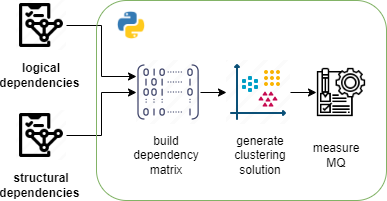
\includegraphics[width=0.8\textwidth]{clustering-generation.png}
    \caption{Clustering solution creation process diagram}
    \label{fig:clustering-gen}
     \end{figure}
\end{center}
\end{frame}

\begin{frame}
\frametitle{Louvain Clustering Algorithm}
\begin{itemize}
    \item Community detection algorithm for complex networks.
    \item Optimizes modularity by moving nodes between clusters.
    \item Suitable for large-scale clustering.
\end{itemize}
\end{frame}

\section{Results}

\begin{frame}
\frametitle{Clustering Results}

In our experiments, for logical dependencies filtering, we started with a strength metric threshold of 10, incrementing in steps of 10 up to 100.
\begin{center}
    \begin{table}
    \centering
    \caption{Louvain Clustering Results - Highlights}
    \begin{tabular}{lccc}
        \toprule
        \textbf{Dataset} & \textbf{Entities} & \textbf{Clusters} & \textbf{MQ Metric} \\
        \midrule
        SD only & 517 & 12 & 0.08 \\
        LD only (Strength 100\%) & 64 & 19 & 0.611 \\
        SD + LD (Strength 30\%) & 517 & 15 & 0.227 \\
        \bottomrule
    \end{tabular}
    \end{table}
\end{center}
\end{frame}


\begin{frame}
\frametitle{Clustering Results: Logical Dependencies Only}
\begin{itemize}
    \item As the strength threshold increases, the number of entities decreases. Higher thresholds filter out more dependencies, leading to fewer entities known by the system.
\end{itemize}
\vspace{-0.5\baselineskip}
\begin{center}
    \begin{table}
    \centering
    \caption{MQ Results for Logical Dependencies Only}
    \begin{tabular}{lccc}
        \toprule
        \textbf{Strength} & \textbf{Entities} & \textbf{Clusters} & \textbf{MQ} \\
        \midrule
	SD only & 517 & 12 & 0.08 \\
	\hline
        10\% & 320 & 56 & 0.506 \\
        20\% & 215 & 53 & 0.547 \\
        30\% & 174 & 44 & 0.558 \\
        40\% & 152 & 40 & 0.580 \\
        50\% & 138 & 35 & 0.604 \\
        60\% & 120 & 34 & 0.587 \\
        70\% & 106 & 32 & 0.577 \\
        80\% & 92 & 29 & 0.576 \\
        90\% & 79 & 24 & 0.606 \\
        \rowcolor{yellow} 100\% & 64 & 19 & \textbf{0.611} \\
        \bottomrule
    \end{tabular}
    \end{table}
\end{center}
\end{frame}

\begin{frame}
\frametitle{Clustering Results: Combined Dependencies}
\begin{center}
    \begin{table}
    \centering
    \caption{MQ Results for Logical + Structural Dependencies}
    \begin{tabular}{lccc}
        \toprule
        \textbf{Strength} & \textbf{Entities} & \textbf{Clusters} & \textbf{MQ} \\
        \midrule
	SD only & 517 & 12 & 0.08 \\
	\hline
        10\% & 517 & 13 & 0.191 \\
        20\% & 517 & 13 & 0.176 \\
        \rowcolor{yellow} 30\% & 517 & 15 & \textbf{0.227} \\
        40\% & 517 & 16 & 0.214 \\
        50\% & 517 & 15 & 0.213 \\
        60\% & 517 & 16 & 0.211 \\
        70\% & 517 & 16 & 0.211 \\
        80\% & 517 & 15 & 0.210 \\
        90\% & 517 & 12 & 0.124 \\
        100\% & 517 & 13 & 0.137 \\
        \bottomrule
    \end{tabular}
    \end{table}
\end{center}
\end{frame}

\section{Discussion}

\begin{frame}
\frametitle{Analysis of Results}
\begin{itemize}
    \item MQ scores for \textbf{LD only} are higher than for \textbf{SD + LD} or \textbf{SD only}.
    \item \textbf{LD only} achieves MQ up to 0.611 at 100\% strength.
    \item However, \textbf{LD only} covers fewer entities (e.g., 64 entities at 100\% strength).
    \item \textbf{SD + LD} covers the entire system (517 entities), a complete coverage.
    \item Balance between clustering quality and system coverage:
    \begin{itemize}
        \item \textbf{LD only}: Better MQ scores but limited coverage.
        \item \textbf{SD + LD}: Lower MQ scores but full system coverage. 
    \end{itemize}
    \item Including logical dependencies improves MQ compared with \textbf{SD only} (MQ: 0.08).
\end{itemize}
\end{frame}


\section{Conclusion}

\begin{frame}
\frametitle{Conclusion}
\begin{itemize}
    \item Incorporating logical dependencies improves clustering quality.
    \item Logical dependencies provide additional insights not available from code analysis alone.
    \item The combined approach leads to clusters with an improved MQ metric and complete system coverage.
\end{itemize}
\end{frame}

\section{Future Work}

\begin{frame}
\frametitle{Future Work}
\begin{itemize}
    \item Expand analysis to more projects.
    \item Explore alternative evaluation metrics and clustering algorithms.
\end{itemize}
\end{frame}

\end{document}
